\section{Análisis del trabajo previo}

\subsection*{Recomendaciones}
\begin{frame}{Recomendaciones de Araujo y Jiménez\footfullcite{ayj}}
\begin{itemize}
  \item Ofrecer Tipos de Dato Abstractos
  \item Permitir la manipulación de apuntadores.
  \item Proveer tipos de dato enumerados.
\end{itemize}
\end{frame}

\subsection*{Mejoras}

\defverbatim[colored]\limits{
\begin{lstlisting}[language=graciela, style=code, escapechar=\~]
var arr : array [5] of int;
write(arr[6]); // Esta línea fallará a tiempo de ejecución
\end{lstlisting}
}

\defverbatim[colored]\multidim{
\begin{lstlisting}[language=graciela, style=code, escapechar=\~]
`var arr : array [5] of array [6] of int;`
`write(arr[3][4]);`
var arr : array [5, 6] of int;
write(arr[3, 4]);
write(arr[3]); // Error a tiempo de compilación
\end{lstlisting}
}

\defverbatim[colored]\inoutarr{
\begin{lstlisting}[language=graciela, style=code, escapechar=\~]
proc p (in a : array [5] of int, out b : array [1~~0] of float)
\end{lstlisting}
}

\begin{frame}{Arreglos}
\framesubtitle{Arreglados}
\begin{itemize}
  \item Se sustituyeron los arreglos de arreglos por arreglos multidimensionales. \multidim{}

  \item Los arreglos ahora pueden ser pasados como parámetros de modo In, In-Out y Out a procedimientos, además del modo Ref. \inoutarr{}

\end{itemize}
\end{frame}
\begin{frame}{Arreglos}
\framesubtitle{Arreglados, cont.}
\begin{itemize}

  \item Se agregó verificación de límites de arreglos, cambiando la estructura interna a una de arreglos conformantes. \limits{} 

  \begin{center}
  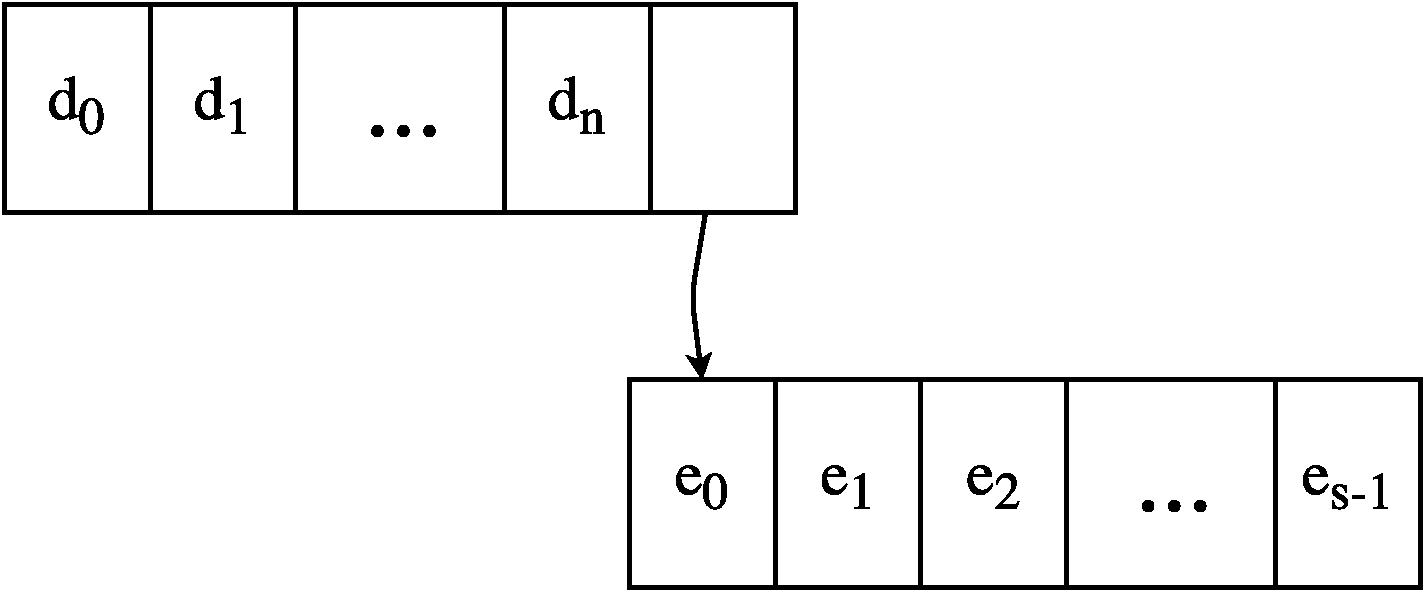
\includegraphics[width=5cm]{diag}
  \end{center}

\end{itemize}
\end{frame}

\defverbatim[colored]\boundproc{
\begin{lstlisting}[language=graciela, style=code, escapechar=\~]
proc p (...)
{pre   ...   pre}
{post  ...  post}
{bound ... bound}
|[ ... p() ... ]|
\end{lstlisting}
}

\defverbatim[colored]\cnfquant{
\begin{lstlisting}[language=graciela, style=code, escapechar=\~]
(% ~\qop~ i : int | 0 < i /\ i < 100 /\ (p(i) \/ q(i)) | ... %)
(% ~\qop~ x : float | x ~\Elem~ xs | ... %)
\end{lstlisting}
}

\defverbatim[colored]\countquant{
\begin{lstlisting}[language=graciela, style=code, escapechar=\~]
(% # i : T | R(i) | P(i) %)
\end{lstlisting}
}

\defverbatim[colored]\constmode{
\begin{lstlisting}[language=graciela, style=code, escapechar=\~]
proc f (const c : int, out r : int) 
    ...
\end{lstlisting}
}

\begin{frame}{Otros cambios}
\begin{itemize}
  \item Los procedimientos y funciones recursivos ahora exigen la definición de una expresión de cota. \boundproc{}

  \item Las cuantificaciones admiten rangos más generales en forma normal conjuntiva. \cnfquant{}
\end{itemize}
\end{frame}

\begin{frame}{Otros cambios}
\begin{itemize}
  \item Se agregó el operador de cuantificación \texttt{count} de Dijkstra\footfullcite{ewd737}. \countquant{}

  \item Se agregó el modo de parámetros Const. \constmode{}

\end{itemize}
\end{frame}
